\documentclass[10pt,conference,compsocconf]{IEEEtran}

\usepackage{hyperref}
\usepackage{graphicx}	% For figure environment
\usepackage{amsmath}
\usepackage{amssymb}
\usepackage{float}
\usepackage{url}
\newcommand{\beginsupplement}{%
	\setcounter{table}{0}
	\renewcommand{\thetable}{S\arabic{table}}%
	\setcounter{figure}{0}
	\renewcommand{\thefigure}{S\arabic{figure}}%
}

\begin{document}
\title{CS-433 Machine Learning Project 2}

\author{
	Matthias Minder, Zora Oswald, Silvan Stettler\\
}

\maketitle

\begin{abstract}
	Abstract...
\end{abstract}

\section*{Introduction} 
The recently developed method of single cell RNA sequencing (scRNA-seq) allows to measure the amount of RNA from a specific gene at the single cell resolution. This gives valuable insight into the properties and cellular function of single cells in a whole population of cells. High throughput methods allow to analyze thousands of cells simultaneously. scRNA-seq results in so-called read-count matrices (RCMs) which indicate the expression level of a given gene in a given cell.
\par 
The emergence of scRNA-seq has led to the discovery of many new cell populations based on their gene expression profile. The question thus naturally arises whether it would be possible to predict cell types using a machine learning approach. To this effect, classifiers can be trained on various publicly available data sets to infer cell types on a new data set \cite{Schwalie2017}. Of special interest is the detection and \textit{de novo} discovery of stem cells in tissues for which no stem cell population has been characterized. It is still unknown whether there exist specific biomarkers for multipotent stem cells allowing to identify them across tissues, which makes this problem attractive to solve. 
\par
However, several challenges are associated with working with scRNA-seq data. The three most predominant issues are the following: Differences in protocols and procedures give rise to batch effects, leading to substantial overall differences between datasets of different sources. Secondly, cell-type annotation is based on clusters of the dataset itself and thus depends on the  analysis and interpretation of the data. This may lead to biases when basing analysis on the annotated clusters. Thirdly, the obtained data is perturbed by so called drop-out events, where the read-counts for a given gene is measured to be zero, even if there were a signal. The result is that RCMs are very sparse. 
\par
Additional issues arise from a machine learning perspective: Since the expression of different genes can be functionally related or controlled by the same transcriptional regulatory program, some features are highly correlated. The scRNA-seq data can thus be thought of as being on a sub-dimensional manifold. However, due to the noisy nature of the data, identifying highly correlated features is difficult. An accurate representation of this manifold is key for obtaining stable results that generalize well to other data sets in order to overcome batch-effects. Moreover, a good such representation also reduces the impact of drop-outs: If several genes are simultaneously expressed for a given biological process, and a subset of these aren't detected due to drop-outs, the other genes could correct this. Naturally, such an approach doesn't work when the drop-out rate is too high. Overall, this nature of scRNA-data suggests that the application of dimensionality reduction prior to method training will yield results that perform better on new, unrelated datasets.
\par
Within this report, we train different stem cell classifiers on multiple published scRNA-seq datasets. The predictive performance is assessed using data from different sources in order to finally determine the best-performing classifier. The presented classifiers are based on different, well-established machine learning methods and were trained on data subjected to different data transformations and dimensionality reduction techniques.

\section*{Methods}
\subsection{Experimental Setup}
For the entire analysis, 17 publicly available scRNA-seq datasets from mature \textit{mus musculus} were used \cite{Campbell2017, Chen2017, Dahlin2018,Dulken2017, Gokce2016, Kowalczyk2015, Haber2017, Hochgerner2018, Rodda2018, Schwalie2018, Nestorowa2016, Park2018, Shah2018, TabulaMuris2017, Tasic2016, Zeisel2018}. These data sets were split into three sets, set A (eleven data sets), set B (three data sets) and set C (four data sets). Two types of classifiers were trained, which will be called basic and nested classifiers. The basic classifiers were trained on set A, and their predictive performance was assessed in terms of the area under the receiver operating characteristic curve (AUC) on the set B and C. The nested classifiers were trained as follows: Using the basic classifiers, predictions were generated for the data in set B. Then, the resulting predictions by all basic classifiers were used as training set for a second classifier, whose performance was assessed and compared with the basic classifiers on set C. By constructing the two-layer nested classifiers, we hoped to be able to obtain a final model which is less prone to batch effects. 
Different basic classifiers were trained on a total of eight data transformations described below, six of which are network-based. 
\begin{table}[H]
	\centering
	\begin{tabular}{|r|c|c|c|}
		\hline
		\textbf{Classifier type} & \textbf{Set A} & \textbf{Set B} & \textbf{Set C} \\ \hline
		Basic & Training & Testing & Testing \\
		Nested & - & Training & Testing \\
		\hline
	\end{tabular}
	\caption{Use of datasets}
\end{table}

\subsection{Dataset Preparation}
Cell type annotation was taken from the clustering done in the original papers. All three sets consist only of cell types which were determined as being clearly stem or non-stem in order to avoid introducing a bias into the model. Notably, progenitors, endothelial and fibroblast cells were excluded from the analysis. For the set A, the cells were down-sampled to be of equal proportions from the three different germ layers, and within each germ layer to be 50\% stem and 50\% non-stem. This was chosen in order to avoid introducing a tissue-specific bias in determining stem-ness. 
\par
Since different datasets measure the expression of different genes, one has to choose which genes to use for the analysis in order to be able to join different datasets. The genes retained for our analysis were selected as follows: For all eleven sets within our train set, we determined whether they contained stem cells, non-stem cells or both. Then, the genes common to all sets with stem-cells were combined with the genes present in all sets containing non-stem cells. In this way, genes that are only expressed in either stem or non-stem cells are retained while minimizing the number of genes with missing values. This resulted in 13'587 genes retained for further analysis.
\par
For datasets in which a necessary gene isn't represented, we set the gene expression to zero. This is based on the heuristic that such genes are lowly expressed in these datasets, as otherwise they would have been sufficiently measured to be retained in the final dataset. 
\par
After retaining only the necessary genes and filling missing values with zero, we normalized the expression values to transcripts per million before transforming the values with $ln(1+x)$. This is standard procedure for scRNA-seq data. All subsequent transformations and training steps were based on data in this format. 

\subsection{Gene Network Construction}
Taking into account external information about the underlying structure is a way to reduce the influence of set specific batch effects. To this effect, we included a protein interaction network, which we then use as topology to process the expression signal. Protein interaction networks are representations of the physical and biochemical interaction between proteins in an organism. The protein interaction network was converted to a gene network by replacing proteins with the genes that encode them. 
\par
The protein interaction data that was used is available in the STRING database (\url{www.string-db.org}) \cite{Szklarczyk2016}. The weight of the edges between individual proteins, which form the nodes, are a measure of how confidently an interaction can be judged to be true. Mapping of genes to their proteins was done using the Ensembl database for \textit{mus musculus} (\url{www.ensembl.org}) \cite{Zerbino2017}. 
For the creation of our network, only the proteins that could be associated to an expressing gene were kept.
Self-loops that resulted from genes whose expression produces multiple proteins and isolated nodes (no link to another node) were removed, yielding a network with 20'330 genes forming nodes that are connected by 11'856'336 edges. It has to be mentioned that the gene network is constructed based on the entire dataset that was available from the sources mentioned above. Contrary to the analysed data, the scope of the network does not limit itself to the genes found in a particular type of cells, such as tissue.  \\

\begin{figure}
	\centering
	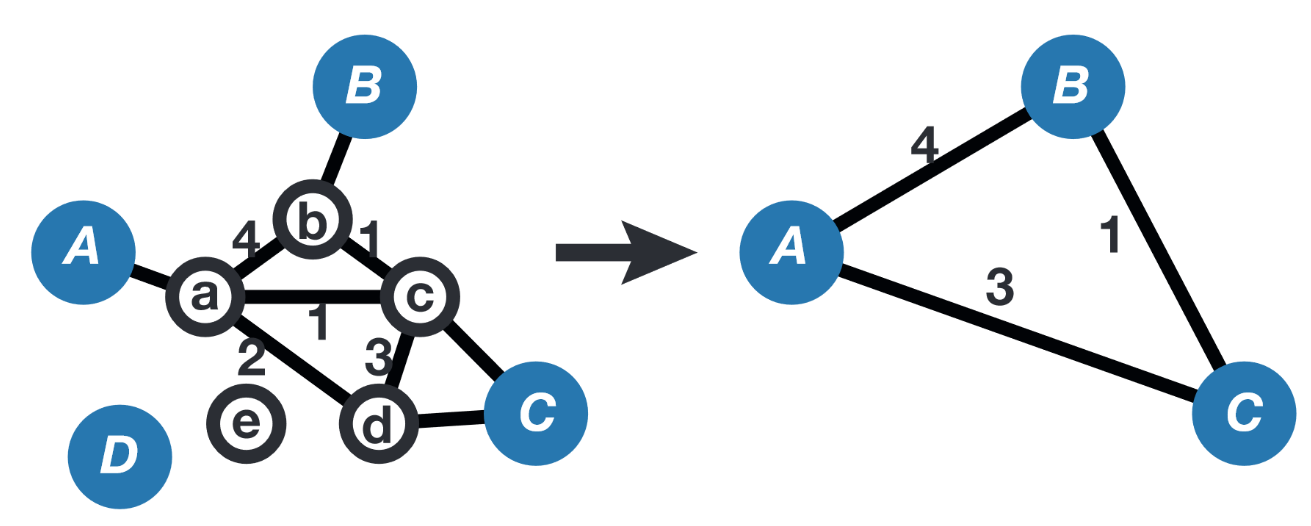
\includegraphics[width=0.45\textwidth]{network.png}
	\caption{Schematic of network creation.  The genes \textit{A, B, C, D} replace the proteins which they express. Proteins that cannot be associated to a gene or vice versa are removed. Resulting self-loops, asi in the case of replacing protein c and d with gene \textit{C} are also removed. Moreover, between gene \textit{A} and \textit{C} two edges of weight 1 and 2 respectively would be created. These edges are summarized in one edge of weight 3. }
	\label{fig:network_creation}
\end{figure}
The process of creating the gene network is schematically shown in Figure \ref{fig:network_creation}. In the case that the replacing of the proteins produces multiple edges between genes, a single edge with a weight equal to the sum of all the individual edge weights is created instead.
\par
The original score $s_{ij}$ of a link between nodes $i$ and $j$ was used to compute an equivalent distance, where high scores result in a short distance. Subsequently, new link weights $W_{ij}$ were set using a Gaussian kernel.

\begin{equation}
W_{ij} = \exp \{- \frac{1}{2}\frac{1}{(s_{ij} \sigma)^2}\}
\end{equation}

\subsection{Feature Creation through Graph Signal Processing}
The scRNA-sec data can be transformed into a graph signal by assigning the count of expressed genes to the corresponding gene in the network, yielding a signal $\boldsymbol{x} \in \mathbb{R}^N$, where $N$ is the total number of nodes. Genes whose expression was not present as a feature in the scRNA-sec data are assigned zero. 
\par
After mapping the data onto the resulting graph, graph signal processing (GSP) can be leveraged to find a lower-dimensional manifold that embeds the original data, based purely on the constructed network. The two methods that were applied take advantage of the fact that the eigendecomposition of the $N \times N$ graph Laplacian matrix $\boldsymbol{L}$ forms the equivalent of a Fourier basis on a graph. Given the eigendecomposition $\boldsymbol{L} = \boldsymbol{U\Lambda U}^T$, $\boldsymbol{U} = [ \boldsymbol{u}_1 ... \boldsymbol{u}_N]$ are the $N$ Fourier basis vectors and the $N$ eigenvalues $\boldsymbol{\Lambda}$ represent the corresponding frequencies.
\par
Graph sampling (GS) is a way to identify genes which are of particular importance to the network. In particular, it identifies nodes where signal energy is the most concentrated for frequencies in the range $(f_{min}, f_{max})$. The \textit{local graph coherence} at node $i$ of order $k$ is defined as the square of the $i$-th entry of the $k$-th eigenvector $u_{ik}$ of the Laplacian, which is a measure for how localized the first $k$ Fourier modes are on node $i$ \cite{Puy2018}. By choosing the first $K$ indices $i$ that maximize $\Sigma_{k=f_{min}}^{f_{max}} u_{ik}^2$, the data can be reduced to the $K$ genes whose read-count information has the most value based on their location in the network for the chosen frequency range. In particular, we applied the GS algorithm for only low frequencies (below $\frac{N}{2}$) and only high frequencies (above $\frac{N}{2}$). 
\par
The idea behind graph frequency sampling (GFS) is essentially to transform the data into the spectral domain and retain components above or below a certain frequency. The Graph Fourier Transform (GFT) $\boldsymbol{\hat{x}}$ of a signal $\boldsymbol{x}$ and its inverse are given by
\begin{align}\label{equ:GFT}
\boldsymbol{\hat{x}} &= \boldsymbol{U}^T \boldsymbol{x}\\ \label{equ:iGFT}
\boldsymbol{x} &= \boldsymbol{U} \boldsymbol{\hat{x}}
\end{align} 
In the GFS algorithm, the graph signal is projected only onto the $K$ eigenvectors associated to eigenvalues below or above a cut-off frequency, resulting in a $K$-dimensional signal $\boldsymbol{\hat{x}_{GFS}}$. For example, choosing the $K$ lowest frequencies,
\begin{equation}
\boldsymbol{\hat{x}_{GFS}} = [ \boldsymbol{u}_1 ... \boldsymbol{u}_K]^T \boldsymbol{x}.
\end{equation} 
\par
We used both the $K$ lowest and highest frequencies separately to transform the original data. GFS using high frequencies (HF) potentially mitigates issues due to batch effects that might appear as a low-frequency component in the graph signal. Similarly, the presence of drop-outs might manifest itself as a high-frequency component and thus be filtered when considering only low-frequency (LF) eigenvectors.
\par
The GFT was also used to implement graph filtering with a simple low or pass rectangle filter in the graph spectral domain. After transforming the data into a graph signal as described previously, the GFT is computed (Equation \ref{equ:GFT}). The components of the resulting spectrum that are above or below a cut-off frequency are set to zero. Subsequently, the inverse GFT (Equation \ref{equ:iGFT}) is applied to obtain a filtered version of the original signal. While this process does not reduce the dimensionality of the data, it could provide insight on validity of the network creation process and reduce noise.
\par

\subsection{Data Transformations}
In summary, 8 different methods are used to transform the data and reduce dimensionality: PCA, Graph sampling (LF and HF), Graph frequency sampling (LF and HF), Graph filtering (LF and HF) and a nested method that combines all the above.

\subsection{Machine Learning Methods}
Within this project, we applied four different types of classifiers to all our data transformations: L1-regularized logistic regression, random forest, neural networks and XGboost.
\par
Logistic regression classifiers were trained using the scikit-learn package in python \cite{scikit-learn}. The regularization parameter was chosen to be the best in accuracy using the built in ten-fold cross-validation functionality using a grid-size of 40. The solution was found using stochastic average descent, with a tolerance of 0.005. 
\par
The random forest classifier was also trained using scikit-learn. For training, 5000 fully grown, unpruned trees were constructed. At every split, $\sqrt{n_{features}}$ were considered when looking for the best split.
\par
Training of XGBoost was done using the python package xgboost \cite{Chen:2016:XST:2939672.2939785}. In order to prevent overfitting, the best classifier was selected based on the best  accuracy on a validation set consisting of 20\% of the training data. A learning rate of 0.2 and a maximum tree depth of three. For all other parameters, default values were used.  
\par
The neural network consists of fully connected layers alternating with ReLU activation functions. It classifies into two classes (non-stem or stem cell) and returns the probabilities using a softmax classifier. Six layers were used for the dimensionality reduced data. Due to a lack of working memory, a hidden layer fc0 with 500 nodes was added at the front of the network for the data with full dimensionality. This allows us to compare the addition of a layer with 500 nodes to a PCA of the same number of dimensions. The architecture is shown in Table \ref{tab:ArchitectureNN} below.

\begin{table}[H]
	\centering
	\begin{tabular}{rccccccc}
\hline
  \textbf{Layer} &  fc0 &  fc1 & fc2 & fc3 & fc4 & fc5 & fc6 \\
  \textbf{Nb Nodes} &  500 &  2500 & 1000 & 200 & 100 & 20 & 2 \\
\hline
\end{tabular}
	\caption{Architecture of the neural network. fc0 is only present for data whose dimensions are not reduced.}
	\label{tab:ArchitectureNN}
	\vspace{-8mm}
\end{table}

The network was trained with stochastic gradient descent on the cross entropy loss in 40 epochs. The best learning rate and regularization constant were found by validating on 15\% of the train set. During the training of the neural network, a learning weight decay was used to avoid oscillating across the optimum.

\section*{Results}
The performance of each classifier was assessed using AUC.
The AUC of the basic classifiers on set B are summarized in Figure \ref{fig:train_acc} below.
\begin{figure}[H]
	\centering
	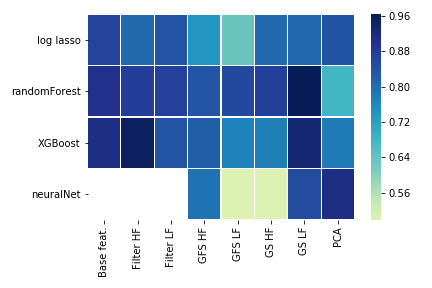
\includegraphics[width=0.45\textwidth]{train_auc.png}
	\caption{AUC scores on set B for the basic classifiers.}
	\label{fig:train_acc}
\end{figure}
We observe that the impact of the choice of data transformation is significant.
The best results were achieved using the network-based GS LF transformation in combination  with maximum AUC of 0.963 for the random forest classifier. Another notable .... The other network-based transformations perform similarly or worse than the baseline model. 
\par  
The following AUC scores were obtained on set C with all classifiers, including the nested classifier that was previously trained on the predictions of the basic classifiers on set B (Figure \ref{fig:train_acc}).

\begin{figure}[H]
	\centering
	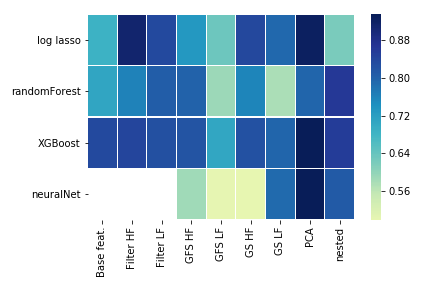
\includegraphics[width=0.45\textwidth]{test_auc.png}
	\caption{AUC scores on set C for all classifiers }
	\label{fig:test_acc}
\end{figure}

While GS LF produced the best results on set B, PCA clearly yield the best AUC scores on set C, outperforming the baseline model with all classifiers. The performance with the network-based dimensionality reduction methods compared to the baseline model is heavily dependent on the choice of classifier. 

Based on the results of set B and C, PCA seems to be the most versatile dimensionality reduction method, producing results that are similar or superior to the baseline model. The scores obtained with the graph-filtered data without dimensionality reduction on set C are similar or higher than the baseline model, but no clear winner between LF and HF can be determined. 

\section*{Conclusion}




%%% Bibliography
\bibliographystyle{IEEEtran}
\bibliography{literature-project2}

\beginsupplement

\begin{table}[H]
	\centering
	\begin{tabular}{rrrrrrrr}
		\hline
		77.0 &  76.7 &  76.1 & 71.4 & 57.6 & 73.1 & 72.4 & 77.2 \\
		76.8 &  75.0 &  77.3 & 76.4 & 75.5 & 77.1 & 81.1 & 76.7 \\
		77.5 &  77.7 &  77.0 & 76.4 & 68.9 & 74.2 & 79.3 & 76.9 \\
		nan   & nan   & nan   & 75.7 & 55.5 & 55.5 & 77.5 & 77.7 \\
		\hline
	\end{tabular}
	\caption{Accuracies on train set, raw data}
\end{table}

\begin{table}[H]
	\centering
	\begin{tabular}{rrrrrrrrr}
		\hline
		66.4 &  83.8 &  80.0 & 65.6 & 59.9 & 77.2 & 66.4 & 85.4 & 53.4 \\
		58.5 &  66.5 &  72.6 & 74.9 & 57.4 & 68.2 & 55.2 & 70.2 & 69.4 \\
		73.9 &  73.8 &  68.5 & 75.3 & 62.2 & 72.9 & 69.0 & 85.1 & 70.0 \\
		nan   & nan   & nan   & 59.1 & 48.3 & 48.3 & 66.4 & 84.7 & 52.6 \\
		\hline
	\end{tabular}
	\caption{Accuracies on test set, raw data}
\end{table}
	

\end{document}
